\makenoidxglossaries
% https://alphabetizer.flap.tv/

\newglossaryentry{API}{name={API}, description={Application Programming Interface.\\ Programmierschnittstelle}}

\newglossaryentry{App}{name={App}, description={Application.\\Programm, welches auf einem Smartphone ausgeführt werden kann. Hier im Besonderen: Ein Teil des von uns entwickelten Produkts als Benutzerschnittstelle}}

\newglossaryentry{ALU}{name={ALU}, 
description={Arithmetic Logic Unit.\\ Das elektronische Rechenwerk eines Prozessors. Es ist speziell konzipiert um mathematische Operationen hocheffizient und schnell durchzuführen}}

\newglossaryentry{ARM}{name={ARM},
description={Acorn RISC Machine, bzw. Advanced RISC Machine.\\ Eine weit verbreitete Mikroprozessorarchitektur, welche sehr oft innerhalb von \gls{SoC}s in \gls{Smartphone}s zum Einsatz kommt}}

\newglossaryentry{CPU}{name={CPU}, 
description={Central Processing Unit.\\ Zentrales Rechen- und Steuerwerk einer Rechenmaschine, hier insb. eines Personalcomputers oder eines Smartphones}}

\newglossaryentry{Data Member}{name={Data Member}, description={~\\Klasseneigenschaft bzw. Membervariable. Eine Variable, die einer Instanz einer Klasse zugeordnet ist und von Instanz zu Instanz variieren kann}}

\newglossaryentry{Deep Learning}{name={Deep Learning}, description={~\\Klasse von Optimierungsmethoden Neuronaler Netzwerke, die zahlreiche Zwischenlagen zwischen Eingabeschicht und Ausgabeschicht haben und dadurch eine umfangreiche innere Struktur besitzen}}

\newglossaryentry{Drehachsen}{name={Drehachsen}, description={~\\Achsen, um die das Smartphone gedreht werden kann. Es gibt die Roll-, Gier- und Nickachse. \begin{figure}[H]
\centering
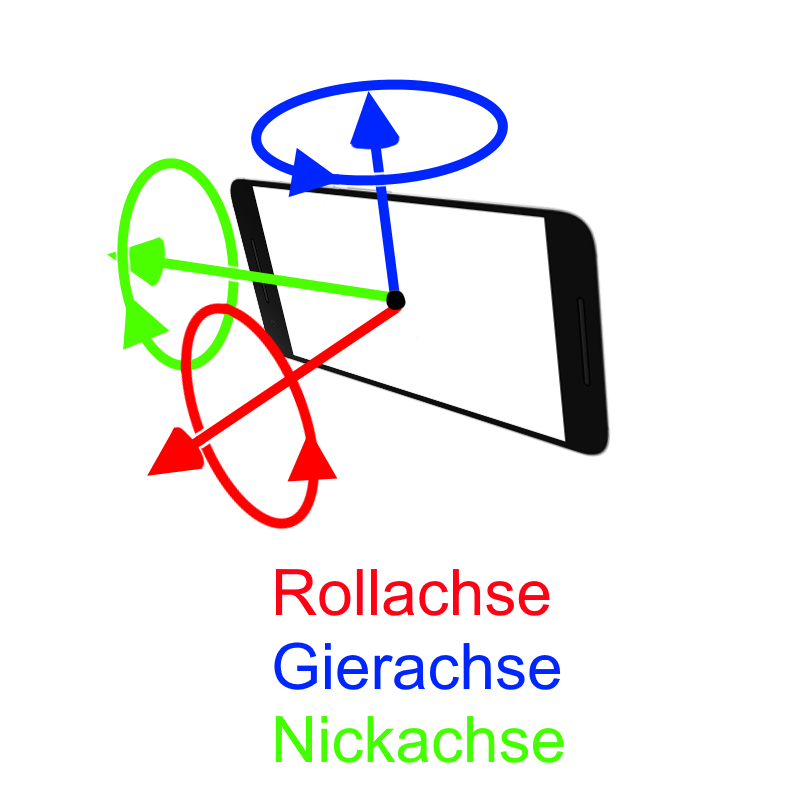
\includegraphics[width=0.5\linewidth]{Reviewdokument/Grafiken/drehachsen.png}
\end{figure}}}

\newglossaryentry{Detektion}{name={Detektion}, description={~\\Lokalisierung eines Merkmals (insb. eines Verkehrszeichens) in einem Bild}}

\newglossaryentry{Fahrzeug}{name={Fahrzeug}, description={~\\Handelsüblicher Personenkraftwagen (PKW), insbesondere kein Lastkraftwagen\\ (LKW)}}

\newglossaryentry{Filter}{name={Filter}, description={~\\Ein Verarbeitungsschritt. Jeder Filter hat eine Dateneingabe und eine -ausgabe. In jedem Verarbeitungsschritt werden die einkommenden Daten umgewandelt. Bei der Umwandlung können den Daten Teile entnommen, hinzugefügt oder auch vollständig ersetzt werden. Die Art der Umwandlung wird durch den Filter bestimmt}}

\newglossaryentry{Filterverwaltungs-Bibliothek}{name={Filterverwaltungs-Bibliothek}, description={~\\Programm-Bibliothek, welche Möglichkeiten bietet, Filter und Neuronale Filter zu laden und auf Bildserien anzuwenden}}

\newglossaryentry{FLOPs}{name={FLOPs}, 
description={Floating Point Operations.\\Operationen auf Fließkommazahlen, die von der \gls{ALU} ausgeführt werden. Sie gelten als eine der aufwendigsten, elementaren Operationen und bestimmen maßgeblich die Laufzeit eines Programms. Ausdrücklich zu unterscheiden von \glqq FLOPS\grqq}}

\newglossaryentry{FLOPS}{name={FLOPS}, 
description={Floating Point Operations per Second.\\Maß für die Leistungsfähigkeit von Computern. Ausdrücklich zu unterscheiden von \glqq FLOPs\grqq}}

\newglossaryentry{Geschwindigkeitsschild}{name={Geschwindigkeitsschild}, description={~\\Gibt die zulässige Höchstgeschwindigkeit des Fahrzeugs an, an dessen Rückseite es befestigt ist. Siehe §58 \gls{StVZO}}}

\newglossaryentry{GPU}{name={GPU}, 
description={Graphics Processing Unit; Grafikkarte.\\ Rechen- und Steuerwerk einer Rechenmaschine, hier insb. eines Personalcomputers oder eines Smartphones, welches auf die Bildverarbeitung spezialisiert ist}}

\newglossaryentry{Keras}{name={Keras}, description={~\\Deep-Learning-Framework in Python basierend auf TensorFlow}}

\newglossaryentry{Klassifikation}{name={Klassifikation}, description={~\\Einteilung eines Merkmals in eine Klasse von Urbildern}}

\newglossaryentry{Konfidenz}{name={Konfidenz}, description={~\\Sicherheit, dass das Objekt korrekt klassifiziert wurde}}

\newglossaryentry{Label}{name={Label}, description={~\\ Meta-Informationen zu einem Sample. In diesem Zusammhang die Position, Größe und Art von Verkehrsschildern in einer Bildaufnahme}}

\newglossaryentry{mAP}{name={mAP}, description={mean Average Precision.\\Maß für die Genauigkeit eines Objekt-Detektors und -Klassifikators. Basiert auf der Position und Größe des vermuteten Bildausschnitts sowie der Rangverteilung der vermuteten Klasse}}

\newglossaryentry{Multithreading}{name={Multithreading}, description={Nebenläufigkeit.\\ Gleichzeitiges Abarbeiten mehrerer Threads innerhalb eines Prozesses}}

\newglossaryentry{Neuronaler Filter}{name={Neuronale Filter}, description={~\\Ein Filter, dessen Umwandlungsvorgehen durch ein Neuronales Netz bestimmt wird}}

\newglossaryentry{Neuronales Netzwerk}{name={Neuronales Netzwerk}, description={~\\Hier im Besonderen: Künstliches Neuronales Netzwerk. Simplifiziertes Modell eines Nervensystems, bestehend aus künstlichen Neuronen, welche auf Computern trainiert werden, um komplexe Aufgaben im Bereich der künstlichen Intelligenz zu bewältigen}}

\newglossaryentry{Nutzer}{name={Nutzer}, description={~\\Der aktuelle Fahrzeugführer, während sich das Fahrzeug nicht in Fahrt befindet bzw. der Beifahrer, während sich das Fahrzeug in Fahrt befindet. Es wird das generische Maskulinum verwendet}}

\newglossaryentry{OpenCV2}{name={OpenCV2}, description={Open Source Computer Vision Library. \\Quelloffene Computergrafikbibliothek. Hier verwendet um Datensätze sowie das erfasste Kamerabild auf die Eingabespezifikationen der Neuronalen Netzwerke anzupassen}}

\newglossaryentry{Produkt}{name={Produkt}, description={~\\Die Kombination aus App und API, welche im Rahmen dieses Softwareprojektes entwickelt werden}}

\newglossaryentry{Pipe}{name={Pipe}, description={~\\Eine Pipe stellt eine Verbindung zwischen den einzelnen Verarbeitungsschritten dar}}

\newglossaryentry{Pipes and Filters}{name={Pipes and Filters}, description={auch Datenfluss-System.\\ Ein Architekturmuster welches die Struktur für Systeme, die Datenströme verarbeiten, darstellt}}

\newglossaryentry{Protobuf}{name={Protocol Buffers, Protobuf}, description={~\\Bezeichnet ein von Google entwickeltes, programmiersprachen- und plattformunabhängiges Format sowie die dazugehörige Implementierung für die Serialisierung und Deserialisierung strukturierter Daten.}}

\newglossaryentry{Sample}{name={Sample}, description={~\\In diesem Zusammenhang eine Bildaufnahme von Verkehrszeichen, welche Neuronalen Netzwerken präsentiert werden können, um sie zur Detektion und Klassifkation zu trainieren}}

\newglossaryentry{Smartphone}{name={Smartphone}, description={~\\Mobiles Endgerät, welches über eine integrierte Kamera verfügt und den im Pflichtenheft spezifizierten Bedingungen genügt}}

\newglossaryentry{SoC}{name={SoC}, description={System-on-a-Chip.\\ Kombination von CPU, Bus, Taktgeber, Co-CPUs, GPU, Soundchip, Interfaces, etc. oder Teilen davon auf einem Chip. Häufig verwendet in mobilen Endgeräten und eingebetteten Systemen um durch hohe Integrationsdichten Fläche auf der Platine einzusparen}}

\newglossaryentry{StVO}{name={StVO}, description={Straßenverkehrsordnung\footlink{https://www.gesetze-im-internet.de/stvo\_2013/StVO.pdf}{29.04.2018}}}

\newglossaryentry{StVZO}{name={StVZO}, description={Straßenverkehrszulassungsordnung\footlink{https://www.gesetze-im-internet.de/stvzo\_2012/StVZO.pdf}{29.04.2018}}}

\newglossaryentry{System}{name={System}, description={~\\Gesamtheit aus Halterung, Smartphone und App}}

\newglossaryentry{Tracking}{name={Tracking}, description={~\\Objekte anhand primitiver Merkmale in einer Bildserie oder einem Video lokalisieren und verfolgen}}

\newglossaryentry{TensorFlow Lite}{name={TensorFlow Lite}, description={~\\Für mobile Endgeräte optimiertes Deep-Learning-Framework des Google Brain Teams\footlink{https://www.tensorflow.org/mobile/tflite/}{29.04.2018}}}

\newglossaryentry{TensorFlow Mobile}{name={TensorFlow Mobile}, description={~\\Deep-Learning-Framework des Google Brain Teams, welches zwar für Android noch keine GPU Unterstützung bietet, dafür aber derzeit noch bzgl. der Kompatibilität besser von bereits etablierten Netzwerken unterstützt wird}}

\newglossaryentry{Tensorflow Node}{name={Tensorflow Node},description={~\\Ein Knoten (Node) im Sinne von TensorFlow bezeichnet eine bestimmte Operation innerhalb des Netzwerk Models: Es ist die grundlegende Einheit für Berechnungen innerhalb von TensorFlow. Die Ergebnisse dieser Knoten lassen sich anhand deren Bezeichnungen (zum Beispiel \glqq{}final\_output\qrqq{})  einzeln abfragen}}

\newglossaryentry{UI}{name={UI},description={User Interface.\\ Benutzeroberfläche}}

\newglossaryentry{VZ}{name={VZ}, description={Verkehrszeichen}}

\newglossaryentry{Verkehrszeichen-API}{name={Verkehrszeichen-API}, description={~\\Besondere Programmierschnittstelle, die für Verkehrszeichenerkennung optimiert ist und erweiterte Logik zur Verfügung stellt, wie etwa die Abschätzung, wann ein Verkehrsschild passiert wurde und damit gültig ist und angezeigt werden muss}}

\newglossaryentry{Verkehrszeichenkombination}{name={Verkehrszeichenkombination}, description={~\\Gruppe von untereinander angebrachten Verkehrszeichen, welche einen gemeinsamen Sinnzusammenhang darstellen}}

\newglossaryentry{VwV-StVO}{name={VwV-StVO}, description={Allgemeine Verwaltungsvorschrift
zur Straßenverkehrs-Ordnung\footlink{http://www.verwaltungsvorschriften-im-internet.de/bsvwvbund\_26012001\_S3236420014.htm}{29.04.2018}}}
